%% Paquetes y configuración %

% Beamer
\PassOptionsToPackage{unicode}{hyperref}  % Evita errores con caracteres no ASCII
\PassOptionsToPackage{naturalnames}{hyperref} % tex.stackexchange.com/questions/10555
\documentclass[compress]{beamer}

% Idioma
\usepackage[spanish]{babel} % Traducciones
\usepackage[utf8]{inputenc} % Uso de caracteres UTF-8
\usepackage{lmodern}        % Fuentes de tamaño arbitrario
\usepackage[T1]{fontenc}    % Permite copiar y evita errores
\uselanguage{Spanish}       % Traducciones beamer
\languagepath{Spanish}      % (tex.stackexchange.com/questions/168208)

% Matemáticas
\usepackage{amsfonts}
\usepackage{amsmath}
\usepackage{amssymb}

% Colores
\definecolor{backg}{HTML}{F2F2F2}    % Fondo
\definecolor{title}{HTML}{bdc3d1}    % Títulos
\definecolor{comments}{HTML}{BDBDBD} % Comentarios
\definecolor{keywords}{HTML}{08388c} % Palabras clave
\definecolor{strings}{HTML}{FA5858}  % Strings
\definecolor{links}{HTML}{2C2C95}    % Enlaces
\definecolor{bars}{HTML}{045FB4}     % Barras (gráfico)

% Código
\usepackage{listings}
\lstset{
language=[LaTeX]TeX,
basicstyle=\footnotesize,
morekeywords={href,uselanguage,languagepath,column},
otherkeywords={pause,usetheme,usecolortheme,useinnertheme,titlepage,tableofcontents,subtitle},
breaklines=true,
backgroundcolor=\color{backg},
keywordstyle=\color{keywords},
commentstyle=\color{comments},
stringstyle=\color{strings},
tabsize=2,
% Acentos, ñ, ¿, ¡ (tex.stackexchange.com/questions/24528)
extendedchars=true,
literate={á}{{\'a}}1 {é}{{\'e}}1 {í}{{\'i}}1 {ó}{{\'o}}1
         {ú}{{\'u}}1 {ñ}{{\~n}}1 {¡}{{\textexclamdown}}1
         {¿}{{?`}}1
}
\lstset{
language=C++,
keywordstyle=\color{blue},
stringstyle=\color{red},
commentstyle=\color{green},
morecomment=[l][\color{magenta}]{\#}
}

% Gráficos
\usepackage{pgfplots}
\pgfplotsset{width=7cm,compat=1.8} % Opciones para gráficos

% Emoticonos
\usepackage{wasysym}

% tikz
\usepackage{tikz}
\usetikzlibrary{mindmap,trees,shadows}
\tikzset{ % Genera overlays
    invisible/.style={opacity=0},
    visible on/.style={alt={#1{}{invisible}}},
    alt/.code args={<#1>#2#3}{\alt<#1>{\pgfkeysalso{#2}}{\pgfkeysalso{#3}}},
}

%% Comandos %%
\newcommand{\ejemplo}[1]{\lstinputlisting{./examples/#1}} % Mostrar código de ejemplos
\newcommand{\muestra}[1]{\input{./examples/#1}}           % Mostrar ejemplos
\newcommand{\seccion}[1]{\input{./sections/#1}}           % Incluir secciones
\newcommand{\espacio}{\vspace*{\baselineskip}}            % Añade espacios
\newcommand{\beamer}{\texttt{beamer} }                    % Estilo único para beamer
\newcommand{\enlace}[3]{\href{#1}{\textbf{#2}} - {\small #3}}  % Estílo único para refs
\newcommand{\comando}[1]{{\color{black}\textbackslash}{\color{keywords}#1}}

%% Temas %%
% Tema y tema de color
  \usetheme{Szeged}
  \usecolortheme{crane}
% \useinnertheme{circles}
  \setbeamercovered{transparent}
% Colores bloques
%  \setbeamercolor{block title}{bg=title,fg=links}
%  \setbeamercolor{block body}{bg=backg,fg=black}
%  \setbeamercolor{block title alerted}{fg=red!70!black,bg=title!92!red}
%  \setbeamercolor{block body alerted}{fg=black,bg=backg}
%  \setbeamercolor{block title example}{fg=green!70!black,bg=title!92!green}
%  \setbeamercolor{block body example}{fg=black,bg=backg}
% Enlaces (tex.stackexchange.com/questions/13423)
\hypersetup{colorlinks,linkcolor=,urlcolor=links}
% Quita enlaces de navegación (stackoverflow.com/questions/3017030)
\setbeamertemplate{navigation symbols}{}
% Quita barra inferior (stackoverflow.com/questions/1435837)
\setbeamertemplate{footline}{}
% Evita warnings boxes
\hfuzz=20pt
\vfuzz=20pt
% Evita wranings itemize
\renewcommand\textbullet{\ensuremath{\bullet}}

% tikz
\usepackage{tikz}
\usetikzlibrary{shapes.multipart}

%% Título y otros %%
\title{Presentación Algoritmos de Ordenación}                                               % Título
\subtitle{Seminario Doble Grado}                                  % Subtítulo
\author{Francisco Gallego Salido}
\institute{Universidad de Granada}
\date{\today}                                                            % Fecha


%%%%%%%%%%%%%%%%%%%%%%%%%%%%%%%%%%%%%%%%%%%%%%%%%%%%%%%%%%%%%%%%

%% Presentación %%
\begin{document}

\begin{frame}
\titlepage
\end{frame}

\begin{frame}
Todo lo necesario está en \href{https://github.com/fgallegosalido}{github.com/fgallegosalido}.\\
\vspace{0.25in}
El programa de la visualización de algoritmos podéis descargarlo \href{https://panthema.net/2013/sound-of-sorting/}{aqu\'i}.
\end{frame}

\begin{frame}{Índice}
  \hypertarget{index}{}
  \tableofcontents
\end{frame}

\section{Introducción}
\subsection{General}

\begin{frame}{General}
	\begin{block}{¿Qué es un algoritmo de ordenación?}
	Un algoritmo de ordenación es un conjunto de pasos que, dada una determinada lista de valores, devuelve la correspondiente lista en orden (de menor a mayor por lo general).
	\end{block}

	\begin{block}{¿Por qué son importantes?}
	Todo sistema informático o aplicación requiere de ordenar algún tipo de datos, ya sean palabras, números o cualquier otra cosa.
	\end{block}
\end{frame}

\subsection{Objetivo}

\begin{frame}{Objetivo}
	\begin{block}{¿Qué vamos a estudiar?}
	Nuestro objetivo en este seminario será el de explicar qué algoritmos de ordenación existen, cuales son mejores, cuales se deben usar y cuales no, calcular su eficiencia, etc.\\
	\vspace{0.20in}
	También aprenderemos a resolver alguna ecuación en recurrencia para poder calcular la eficiencia de algoritmos recursivos.\\
	\vspace{0.20in}
	Todo esto irá acompañado de gráficas (que vosotros mismos podréis generar) para corroborar todo lo aprendido.
	\end{block}
Empecemos pues...
\end{frame}

\section{Eficiencia}
\subsection{Concepto}

\begin{frame}{¿Qué es la eficiencia?}
	\begin{block}{Definición}
	La eficiencia de un algoritmo es básicamente la velocidad del mismo a medida que el número de datos crece. Para representar la eficiencia usaremos la notación O-grande $\mathcal{O}(f)$, donde f es el orden de eficiencia.\\
	\vspace{0.20in}
	En las siguientes diapositivas explicaremos en qué consiste esta notación y qué propiedades tiene.
	\end{block}
\end{frame}

\begin{frame}{¿Para qué sirve?}
La eficiencia nos servirá para poder decidirnos a la hora de elegir algoritmos e implementarlos.\\
\vspace{0.20in}
Podríamos decir que, computacionalmente hablando, siempre vamos a intentar elegir aquellos algoritmos cuyo orden de eficiencia sea menor, es decir, la función de eficiencia crece más lentamente.\\
\vspace{0.20in}
	\begin{exampleblock}{Ejemplo}
	Supongamos que el algoritmo 1 tiene orden $\mathcal{O}(n^2)$ y el algoritmo 2 $\mathcal{O}(2^n)$. En este caso eligiremos el algoritmo 1, pues su orden de eficiencia es menor (después explicaremos por qué).
	\end{exampleblock}
\end{frame}

\subsection{Notación $\mathcal{O}$}

\begin{frame}{Representación}
Como ya hemos dicho anteriormante, el orden de una función (en nuestro caso lo usaremos para el orden de eficiencia) se expresa mediante la notación O-grande o $\mathcal{O}(f)$, donde f es una función que determina el orden.\\
\vspace{0.20in}
	\begin{exampleblock}{Ejemplos}
	$\mathcal{O}(n)$, $\mathcal{O}(2^n)$, $\mathcal{O}(n^4)$, $\mathcal{O}(\log_2(n))$, $\mathcal{O}(n\log_2(n))$ ...
	\end{exampleblock}
\end{frame}

\begin{frame}{Función de orden}
Las funciones de orden no son como las funciones que conocemos, sino más bien una simplificación de las mismas, donde solo nos interesa cómo crecen. Vamos a poner un ejemplo:
	\begin{exampleblock}{Ejemplo}
	Si tenemos que $f(x) = 3x^4 + 5x^2 + x + 4$, entonces el orden de esta función se corresponde con el término dominante, es decir, el que crece más rápido, sin constantes, es decir, el orden de $f(x)$ es $\mathcal{O}(n^4)$.
	\end{exampleblock}
\end{frame}

\begin{frame}{¿Qué funciones tienen mayor orden?}
Como es natural, es necesario poder ordenar dichas funciones para así decidir cuál es el término que crece más rápido.\\
\vspace{0.20in}
	\begin{block}{Definición}
	Dadas dos funciones $f(x)$ y $g(x)$, diremos que $\mathcal{O}(g) < \mathcal{O}(f)$ si $\nexists r\in \mathbb{R}$ tal que $f(x) < r\cdot g(x)$ $\forall x\in \mathbb{R}$
	\end{block}
\end{frame}

\begin{frame}{Ejemplos}
Vamos a poner un ejemplo.\\
\vspace{0.20in}
	\begin{exampleblock}{Ejemplo}
	$f(x) = 2^x$, $g(x) = 3^x$. Es evidente que $\mathcal{O}(g) < \mathcal{O}(f)$ porque $3^x < r\cdot2^x \Rightarrow (\tfrac{3}{2})^x < r$, pero \[\lim_{x \to +\infty}(\tfrac{3}{2})^x = \infty\]luego  no existe ninguna constante r que acote ese límite.
	\end{exampleblock}

	\begin{alertblock}{Cuidado}
	Si tenemos $f(x) = x^2$ y $g(x) = 1000000x^2$, $\mathcal{O}(g) = \mathcal{O}(f)$ por muy grandes que sean las constantes de $g(x)$.
	\end{alertblock}
\end{frame}

\begin{frame}{Operaciones}
Una vez conocida la notación, vamos a ver las dos operaciones básicas:
	\begin{itemize}
	\item Suma: $\mathcal{O}(f) + \mathcal{O}(g) = \mathcal{O}(\max(f,g))$
	\item Producto: $\mathcal{O}(f) \cdot \mathcal{O}(g) = \mathcal{O}(f\cdot g)$
	\end{itemize}

	\begin{exampleblock}{Ejemplos}
	$\mathcal{O}(n) + \mathcal{O}(\log_2(n)) = \mathcal{O}(n)$\\
	$\mathcal{O}(n) \cdot \mathcal{O}(2^n) = \mathcal{O}(n\cdot2^n)$
	\end{exampleblock}
\vspace{0.20in}
Ya tenemos todo lo necesario para calcular algunas eficiencias.
\end{frame}

\subsection{Cálculo de eficiencia}

\begin{frame}[fragile]{Código Sin Bucles}
Consideremos este código:\\
\vspace{0.20in}
	\begin{lstlisting}
	#include <iostream>
	int main(){
	  int a, b=0, aux;
	  std::cin >> a;
	  aux = a;
	  a = b;
	  b = aux;

	  std::cout << a << b << std::endl;
	}
	\end{lstlisting}
\end{frame}

\begin{frame}[fragile]{Solución Código Sin Bucles}
Cada instrucción se considera $\mathcal{O}(1)$:
	\begin{lstlisting}
	#include <iostream>
	int main(){
	  int a, b=0, aux;  //------------------->O(1)
	  std::cin >> a;  //--------------------->O(1)
	  aux = a;  //--------------------------->O(1)
	  a = b;  //----------------------------->O(1)
	  b = aux;  //--------------------------->O(1)

	  std::cout << a << b << std::endl;  //-->O(1)
	}
	\end{lstlisting}
Sumamos todos los órdenes y listo, luego el orden de este código sería $\mathcal{O}(1)$.
\end{frame}

\begin{frame}[fragile]{Código Con Bucles}
Consideremos este otro código:\\
\vspace{0.20in}
	\begin{lstlisting}
	#include <iostream>
	int main(){
	  int n;
	  std::cin >> n;
	  int* v = new int[n];

	  for (int i=0; i<n; ++i){
	    v[i] = i;
	  }
	}
	\end{lstlisting}
\end{frame}

\begin{frame}[fragile]{Solución Código Con Bucles}
La eficiencia de un bucle es la eficiencia de lo que hay dentro por el número de iteraciones del bucle:\\
\vspace{0.20in}
	\begin{lstlisting}
	#include <iostream>
	int main(){
	  int n;  //--------------------------->O(1)
	  std::cin >> n;  //------------------->O(1)
	  int* v = new int[n];  //------------->O(1)

	  for (int i=0; i<n; ++i){//      |\
	    v[i] = i;  //----------->O(1) |---->O(1)*n = O(n)
	  }//                             |/
	}
	\end{lstlisting}
Sumamos todos los órdenes y listo, luego el orden de este código sería $\mathcal{O}(n)$.
\end{frame}

\begin{frame}[fragile]{Código Con Recursividad}
Consideremos este otro código:\\
\vspace{0.20in}
	\begin{lstlisting}
	int Bar(int* array, int size, int ini, int fin){
	  if(n>1){
	    Bar(array, size-1, ini, fin-1);  //Llamada a todos menos al último
	    Bar(array, size-1, ini+1, fin);  //Llamada a todos menos al primero
	  }
	}
	\end{lstlisting}
\end{frame}

\begin{frame}[fragile]{Solución Código Con Recursividad}
La eficiencia para la recursividad ha de resolverse con una ecuación recurrente:\\
\vspace{0.20in}
	\begin{lstlisting}
	int Bar(int* array, int size, int ini, int fin){
	  if(n>1){
	    Bar(array, size-1, ini, fin-1);  //------>O(?)
	    Bar(array, size-1, ini+1, fin);  //------>O(?)
	  }
	}
	\end{lstlisting}
Para plantear esta ecuación, solo nos vamos a centrar en las dos llamadas a la funciones Bar.
\end{frame}

\subsubsection{Cálculo de Ecuaciones en Recurrencia}

\begin{frame}{Ecuación Recurrente}
Suponiendo $n$ el tamaño del vector que se pasa y $T(n)$ la función que determina la eficiencia, podemos plantearla de la siguiente manera:\\
\vspace{0.20in}
	\begin{block}{Ecuación}
	\[
	T(n) = \left\{
	\begin{array}{l l}
	1 & if \quad n=1\\
	2T(n-1) & if \quad n>1\\
	\end{array} \right. \]
	\end{block}
La técnica que vamos a seguir para este caso va a ser expandir la ecuación e ir deduciendo cosas. Hay otros métodos según la ecuación a resolver, pero por el momento nos conformamos con este.
\end{frame}

\begin{frame}{Solución Ecuación Recurrente}
Vamos expandiendo la ecuación:\\
\vspace{0.20in}
$T(n) = 2T(n-1) = 2\cdot(2T(n-2)) = 2^2\cdot T(n-2) =$\\
$= 2^2\cdot(2T(n-3)) = 2^3\cdot T(n-3) =$...\\
\vspace{0.20in}
Como podemos ver, al expandir aparece cierto patrón, que en general se tiene $T(n) = 2^i\cdot T(n-i)$. Vamos a tomar $i=n-1$:\\
\vspace{0.20in}
$T(n) = 2^{n-1}\cdot T(n-(n-1)) = 2^{n-1}\cdot T(1) = 2^{n-1}$\\
\vspace{0.20in}
Luego $T(n) = 2^{n-1}$, lo que implica que el orden de dicho algoritmo es $\mathcal{O}(2^n)$ (no $\mathcal{O}(2^{n-1})$).
\end{frame}

\section{Algoritmos de Ordenación}
\subsection{Índice de Algoritmos}

\begin{frame}{Categorías}
Y empezamos con la parte que realmente nos interesa, los algoritmos de ordenación y sus técnicas. Los vamos a dividir como sigue:\\
	\begin{itemize}
	\item Algoritmos cuadráticos\\
		\begin{itemize}
		\item Burbuja
		\item Selección
		\item Inserción
		\end{itemize}
	\item Algoritmos Divide y Vencerás\\
		\begin{itemize}
		\item Mergesort
		\item Quicksort
		\item Bitonicsort
		\end{itemize}
	\end{itemize}
\end{frame}

\begin{frame}{Categorías}
	\begin{itemize}
	\item Algoritmos de Ordenación por Conjuntos\\
		\begin{itemize}
		\item RadixsortLSD
		\item RadixsortMSD
		\item Countingsort
		\end{itemize}
	\item Algoritmos Varios\\
		\begin{itemize}
		\item Heapsort
		\item Timsort
		\item Slowsort
		\item Permutationsort
		\item Bogosort
		\end{itemize}
	\end{itemize}
\end{frame}

\subsection{Cuadráticos}

\begin{frame}{Introducción}
	\begin{block}{¿Cuáles son?}
	Lo algoritmos cuadráticos son aquellos cuya eficiencia es $\mathcal{O}(n^2)$.
	\end{block}
\vspace{0.20in}
	\begin{block}{¿Qué utilidad tienen?}
	Realmente estos algoritmos tienen poca utilidad práctica, pues son extremadamente lentos comparados con otros que veremos más adelante. Aún así alguno se comporta muy bien con muy pocos elementos o con vectores casi ordenados.
	\end{block}
\end{frame}

\begin{frame}{Burbuja}
Este algoritmo consiste básicamente en ir trasladando el máximo de los elementos que aún no están ordenados al principio de los que sí están ordenados.\\
\vspace{0.20in}
Podríamos decir que este es el peor de los algoritmos cuadráticos y que solo es útil para fines académicos.\\
\vspace{0.20in}
	\begin{block}{Eficiencia}
	En el mejor caso, cuando el primer elemento es el mayor de todos y los demás están ordenados, es $\mathcal{O}(n)$; en el caso peor y promedio es $\mathcal{O}(n^2)$
	\end{block}
\end{frame}

\begin{frame}{Gráfica}
	\begin{alertblock}{}
		\begin{center}
		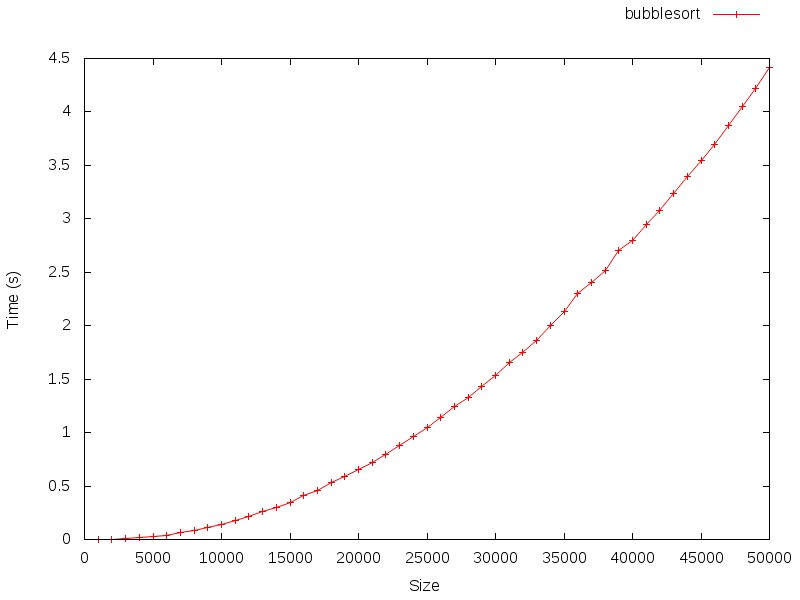
\includegraphics[scale=0.40]{images/bubblesort.jpeg}
		\end{center}
	\end{alertblock}
\end{frame}

\begin{frame}{Selección}
Este algoritmo es parecido al de Burbuja pero al revés, es decir, busca el mínimo de los que no están ordenados y lo inserta al final de los ordenados.\\
\vspace{0.20in}
Tampoco es una maravilla comparado con el Burbuja (de hecho en las gráficas es peor que el burbuja).\\
\vspace{0.20in}
	\begin{block}{Eficiencia}
	En el caso mejor, peor y promedio es $\mathcal{O}(n^2)$.
	\end{block}
\end{frame}

\begin{frame}{Gráfica}
	\begin{alertblock}{}
		\begin{center}
		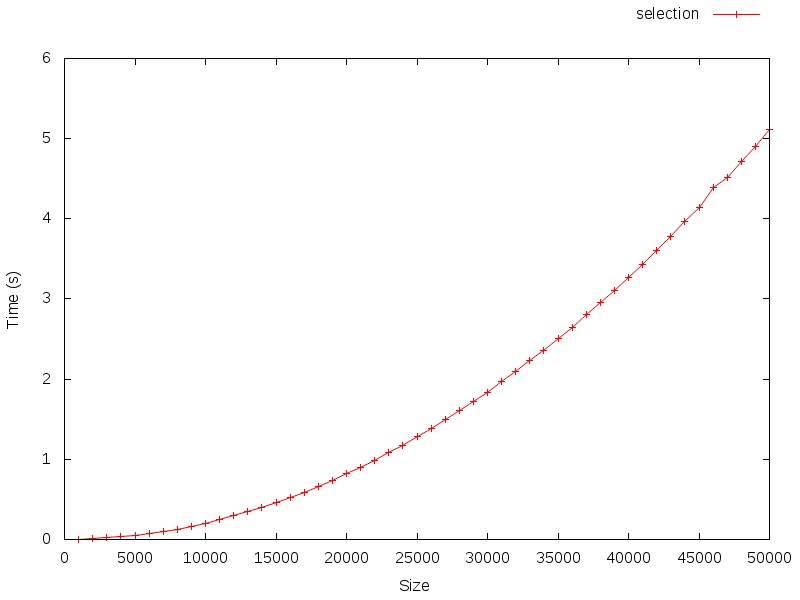
\includegraphics[scale=0.40]{images/selection.jpeg}
		\end{center}
	\end{alertblock}
\end{frame}

\begin{frame}{Inserción}
Este algoritmo consiste en ir recorriendo el vector de los elementos que no están ordenados e insertarlo en su correspondiente sitio en los ordenados.\\
\vspace{0.20in}
Este algoritmo, al contrario que los otros dos cuadráticos, sí que se usa en algunas situaciones. Por ejemplo, con pocos elementos tiene mejores resultados que algunos de los más rápidos como el Quicksort, por lo que a partir de cierto umbral se usa este.\\
\vspace{0.20in}
	\begin{block}{Eficiencia}
	En el caso mejor es $\mathcal{O}(1)$, y en el peor y promedio es $\mathcal{O}(n^2)$, aunque en algunas situaciones concretas tiende a tener una eficiencia $\mathcal{O}(n)$.
	\end{block}
\end{frame}

\begin{frame}{Gráfica}
	\begin{alertblock}{}
		\begin{center}
		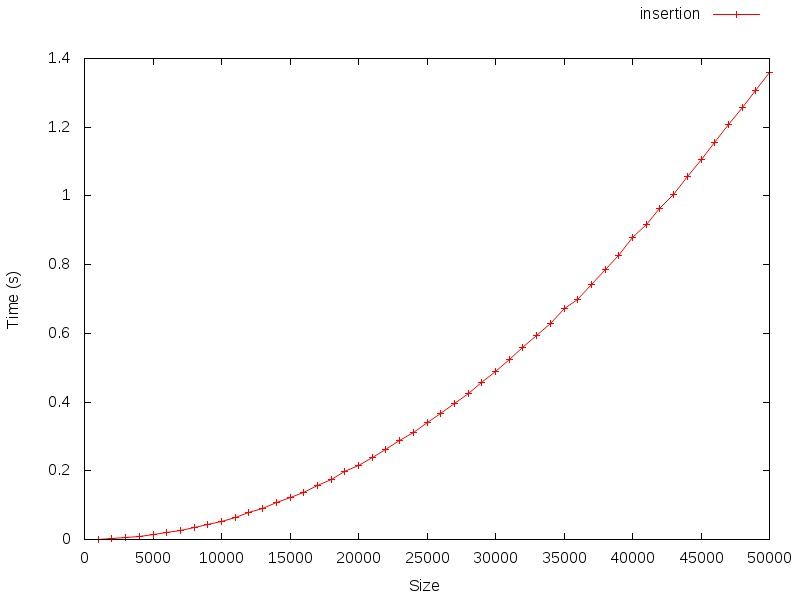
\includegraphics[scale=0.40]{images/insertion.jpeg}
		\end{center}
	\end{alertblock}
\end{frame}

\begin{frame}{Comparación Cuadráticos}
	\begin{alertblock}{}
		\begin{center}
		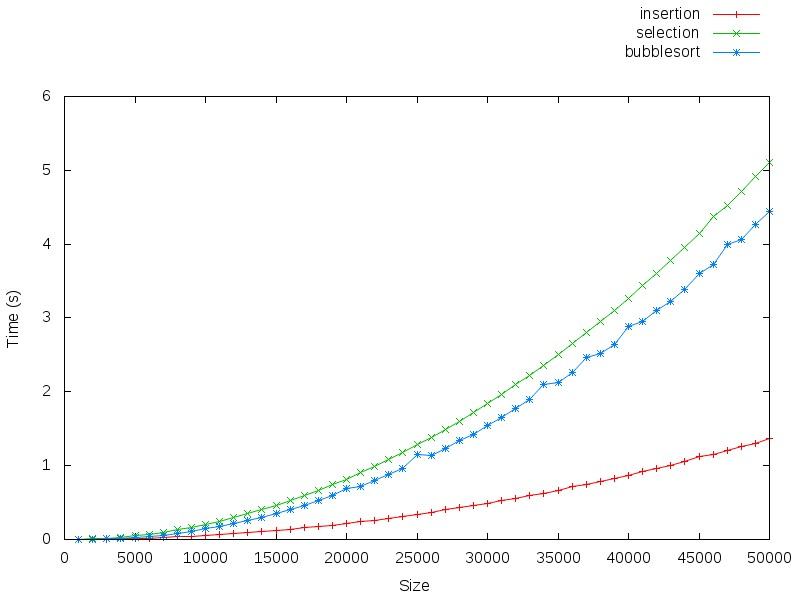
\includegraphics[scale=0.40]{images/slow.jpeg}
		\end{center}
	\end{alertblock}
\end{frame}

\subsection{Divide y Vencerás}

\begin{frame}{Introducción}
	\begin{block}{¿Cuáles son?}
	Estos algoritmos son aquellos que siguen la filosofía de "Divide y Vencerás", la cual explicaremos a continuación. Suelen tener eficiencia más o menos próxima a $\mathcal{O}(n\cdot\log_2(n))$.
	\end{block}
\vspace{0.20in}
	\begin{block}{¿Qué utilidad tienen?}
	Son los algoritmos que se utilizan en los sistemas reales, pues son muy rápidos y pueden trabajar con cualquier tipo de datos, ya sean palabras, números, letras o cualquier cosa que pueda ser comparada.
	\end{block}
\end{frame}

\subsubsection{Técnica "Divide y Vencerás"}

\begin{frame}{Filosofía}
	\begin{columns}
		\begin{column}{4.3cm}
			\begin{block}{¿En qué consiste?}
			Esta técnica consiste en dividir el problema total en problemas más pequeños y fáciles de resolver.\\
			\vspace{0.20in}
			Una vez se han resuelto estos problemas, se unen las soluciones para generar la solución al problema total. Podemos verlo en el esquema de la imagen.
			\end{block}
		\end{column}
		\begin{column}{6cm}
			\begin{alertblock}{}
			\hspace*{+0.5cm}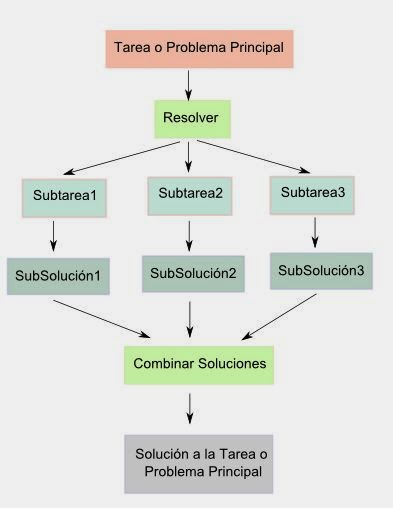
\includegraphics[scale=0.36]{images/metodo_divide_y_venceras.JPG}
			\end{alertblock}
		\end{column}
	\end{columns}
\end{frame}

\begin{frame}{Mergesort}
El primer algoritmo que vamos a tratar va a ser el Mergesort. Este algoritmo divide el vector en dos partes de igual tamaño. Esto lo hace recursivamente. Podemos decir que esta es la parte de división del trabajo.\\
\vspace{0.20in}
Una vez llegado el caso base, se van uniendo las mitades (estas ya ordenadas) con una función de fusión (la cual ahora explicaré) de manera que la parte resultante queda ordenada.\\
\vspace{0.20in}
	\begin{block}{Eficiencia}
	La eficiencia de este algoritmo es siempre $\mathcal{O}(n\cdot\log_2(n))$, aunque con pocos elementos tal vez convenga más usar algún otro algoritmo de ordenación (como el inserción).
	\end{block}
\end{frame}

\begin{frame}{Gráfica}
	\begin{alertblock}{}
		\begin{center}
		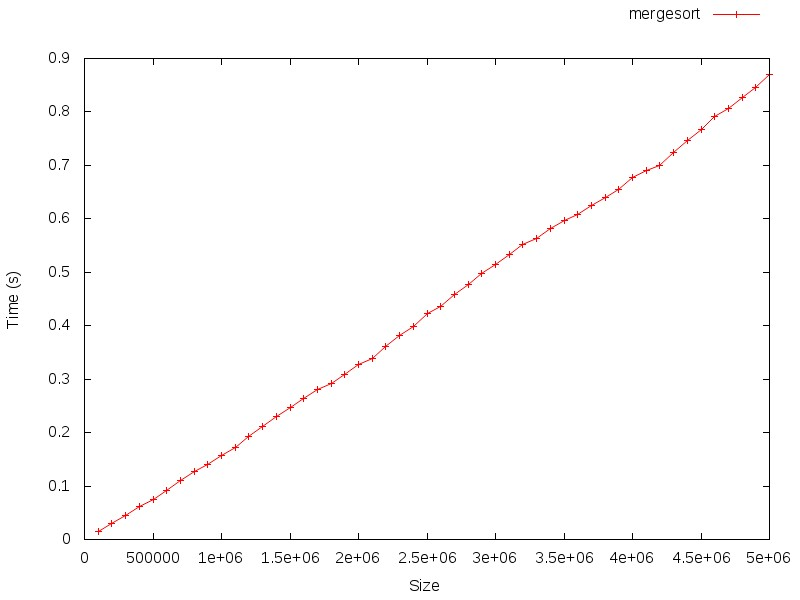
\includegraphics[scale=0.40]{images/mergesort.jpeg}
		\end{center}
	\end{alertblock}
\end{frame}

\begin{frame}{Quicksort}
Llegamos al que posiblemente sea el algoritmo más usado de todos. Este algoritmo sigue estos pasos:\\
\vspace{0.20in}
	\begin{itemize}
	\item Selecciona un pivote, esto es, un elemento al azar del vector.
	\item Cambia elementos de manera que a la izquierda del pivote todos son menores que el pivote, y a la derecha mayores.
	\item Aplica Quicksort sobre ambas particiones del vector
	\end{itemize}
\vspace{0.20in}
	\begin{block}{Eficiencia}
	Si hay que ponerle un pero al algoritmo es lo aleatorio de la partición. En el mejor caso y en el promedio tiene eficiencia $\mathcal{O}(n\cdot\log_2(n))$, pero en el peor caso nos vamos a la horrible eficiencia de $\mathcal{O}(n^2)$, que se dará cuando siempre que se elija un pivote, sea el menor o mayor del vector.
	\end{block}
\end{frame}

\begin{frame}{Gráfica}
	\begin{alertblock}{}
		\begin{center}
		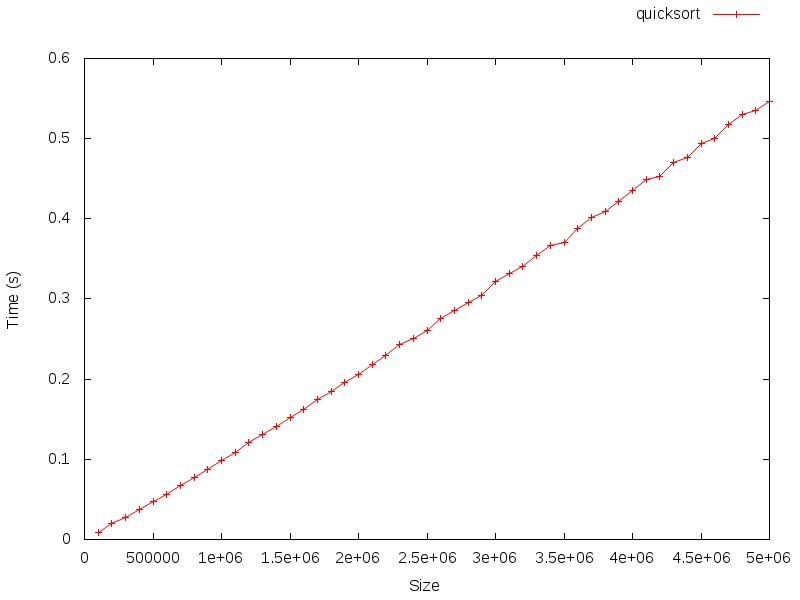
\includegraphics[scale=0.40]{images/quicksort.jpeg}
		\end{center}
	\end{alertblock}
\end{frame}

\begin{frame}{Comparación Mergesort-Quicksort}
	\begin{alertblock}{}
		\begin{center}
		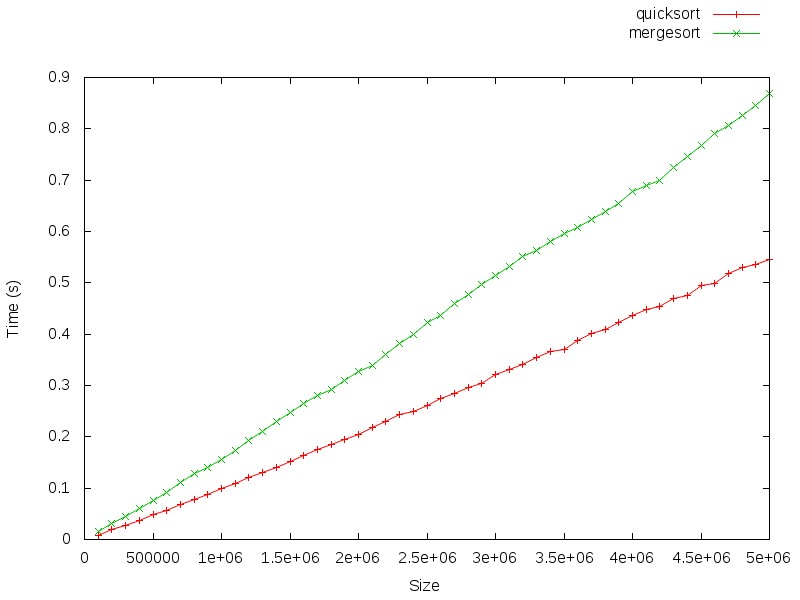
\includegraphics[scale=0.40]{images/quic-merg.jpeg}
		\end{center}
	\end{alertblock}
\end{frame}

\begin{frame}{Bitonicsort}
Ahora hablaremos de un algoritmo un tanto desconocido, pero que sin embargo es muy usado en computación paralela debido a la facilidad de paralelizar las divisiones.\\
\vspace{0.20in}
Es parecido al Mergesort, pero este algoritmo hace la fusión de una manera que permite la paralelización. Consiste en:\\
\vspace{0.20in}
	\begin{itemize}
	\item Hace la división en mitades, igual que el mergesort.
	\item Cada mitad se ordena diferente: una creciente y otra decreciente, formando lo que se conoce como una secuencia bitónica.
	\item Se aplica la función de fusión, al igual que con el mergesort, con la particularidad de que esta sí que puede ser paralelizada.
	\end{itemize}
\end{frame}

\begin{frame}{Bitonicsort}
Puesto que es un algoritmo algo difícil de comprender, se explicará la idea para $n = 2^k$ datos (para un número arbitrario de datos se usa una ligera modificación de esta idea, pero más pulida).\\
\vspace{0.20in}
	\begin{block}{Eficiencia}
	En el caso secuencial (sin paralelizar), este algoritmo tendrá una eficiencia media de $\mathcal{O}(n\cdot\log_2(n)^2)$, pero como normalmente se usa en paralelo, la eficiencia desciende según el número de procesadores, generalizando a que, suponiendo que hay $n$ procesadores, la eficiencia sería $\mathcal{O}(log_2(n)^2)$, aunque en la práctica realmente sea $\mathcal{O}((\tfrac{n}{k})log_2(n)^2)$, siendo $k$ el número de procesadores.
	\end{block}
\end{frame}

\begin{frame}{Gráfica}
	\begin{alertblock}{}
		\begin{center}
		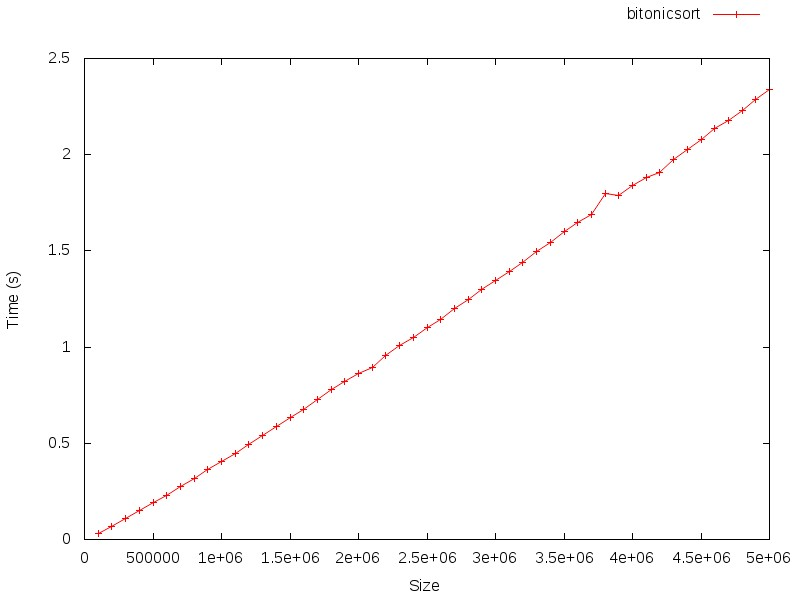
\includegraphics[scale=0.40]{images/bitonicsort.jpeg}
		\end{center}
	\end{alertblock}
\end{frame}

\begin{frame}{Comparación Divide y Vencerás}
	\begin{alertblock}{}
		\begin{center}
		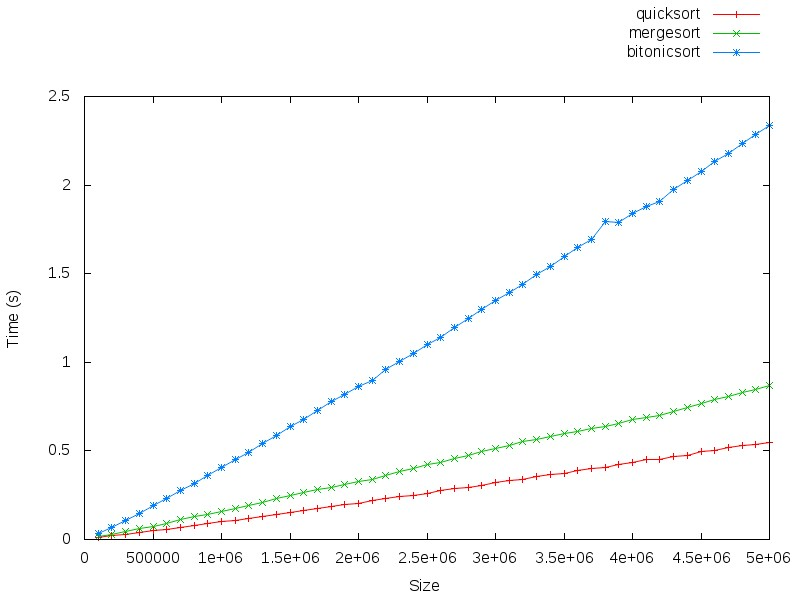
\includegraphics[scale=0.40]{images/quic-merg-bito.jpeg}
		\end{center}
	\end{alertblock}
\end{frame}

\subsection{Ordenación por Conjuntos}

\begin{frame}{Introducción}
	\begin{block}{¿Cuáles son?}
	Estos algoritmos son aquellos en los que se ordena por conjuntos o separando, de tal modo que no son necesarias comparaciones entre dos elementos cualesquiera.
	\end{block}
\vspace{0.20in}
	\begin{block}{¿Qué utilidad tienen?}
	Son los algoritmos más rápidos en casos concretos, llegando a alcanzar órdenes de eficiencia de $\mathcal{O}(n)$. Esto es debido a que se aprovechan ciertas propiedades de los datos (como que estos sean números enteros o que no sean negativos) para idear algoritmos pensados para tratar esos tipos de datos.
	\end{block}
\end{frame}

\begin{frame}{Radixsort}
El Radixsort es un algoritmo que ordena según los dígitos de los datos (es decir, enteros no negativos). Tiene dos variantes\\
	\begin{itemize}
	\item Dígito Menos Significativo (LSD): Va ordenando empezando por los dígitos menos significativos (unidades, decenas...) hacia los más significativos (millón, decena de millón...).
	\item Dígito Más Significativo (MSD): Justo al revés que el anterior, solo que para este caso es necesaria la recursividad y para el anterior no.
	\end{itemize}
	\begin{block}{Eficiencia}
	La eficiencia de este algoritmo depende del dato que se esté ordenando. Suponiendo que el tamaño del dato en bits es $w$, la eficiencia sería $\mathcal{O}(w\cdot n)$. Puesto que el $w$ es constante a lo largo del algoritmo, podemos asumir que el orden es $\mathcal{O}(n)$, aunque con unas constantes ocultas un tanto altas.
	\end{block}
\end{frame}

\begin{frame}{Radixsort}
La idea general del LSD es ir recorriendo el vector e ir metiendo los datos en conjuntos diferentes según el dígito que se esté comprobando (si es $1$ va al conjunto A, si es $2$ va al conjunto B...) y luego sacar todos los del conjunto A primero en el mismo orden que han entrado, después los del B y así hasta el último conjunto. Al repetir esto con dígitos cada vez más significativos, acabaremos con un vector ordenado.\\
\vspace{0.20in}
Para el MSD hacemos lo mismo solo que empezando por el dígito más significativo, y luego llamamos recursivamente en cada conjunto por separado.\\
	\begin{exampleblock}{Nota}
	Tal vez interese usar colas como conjuntos...
	\end{exampleblock}
\end{frame}

\begin{frame}{Comparación LSD-MSD}
	\begin{alertblock}{}
		\begin{center}
		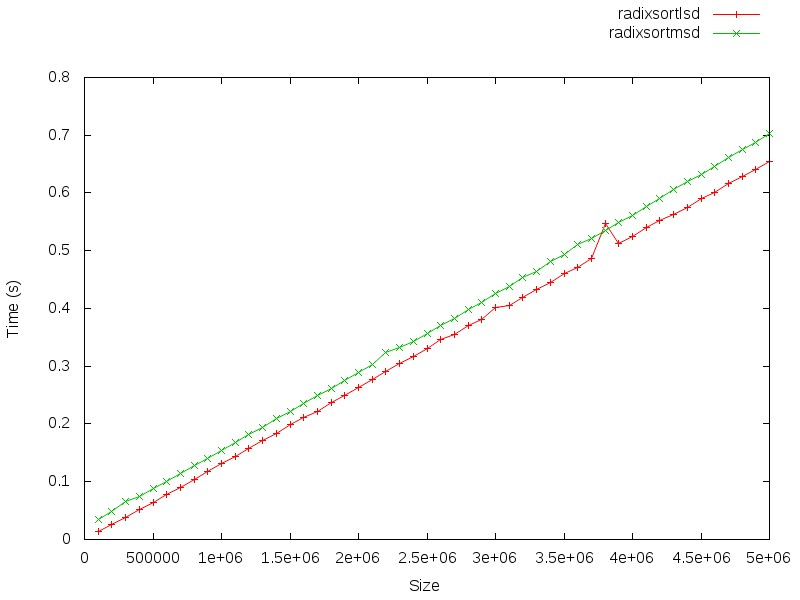
\includegraphics[scale=0.40]{images/radi-radi.jpeg}
		\end{center}
	\end{alertblock}
\end{frame}

\begin{frame}{Countingsort}
Este, al menos en los que hay implementados, es el más rápido de todos con números enteros y por diferencia. La idea es sumamente simple, aunque muy restringida a que sean enteros (si no lo son, el algoritmo falla de mala manera, cosa que puede no pasarle al radixsort).\\
\vspace{0.20in}
Consiste en crear un vector auxiliar de tamaño igual a la diferencia entre el mayor y el menor del vector dado(notar que si hay mucha diferencia, el algoritmo puede no ser muy eficiente). Suponiendo que el mínimo es $1$ y el máximo $10$, nuestro vector auxiliar tendrá tamaño $10$. Lo que hacemos es, en la posición $x$ del vector meter la cantidad de veces que aparece ese mismo número en el vector dado, y luego volcar el vector auxiliar en el original.
\end{frame}

\begin{frame}{Countingsort}
	\begin{block}{Eficiencia}
	La eficiencia de este algoritmo es en general $\mathcal{O}(n)$ para una distribución más o menos uniforme. Sin embargo, puede dar resultados muy malos si, por ejemplo, tenemos solo 10 datos a ordenar pero el menor es 1 y el mayor 1000000, en cuyo caso pierde mucha velocidad con respecto al número de datos.
	\end{block}
\vspace{0.20in}
En la gráfica comparativa de los tres algoritmos de ordenación por conjuntos y en la final se verá claramente que este es el más rápido y con diferencia
\end{frame}

\begin{frame}{Gráfica}
	\begin{alertblock}{}
		\begin{center}
		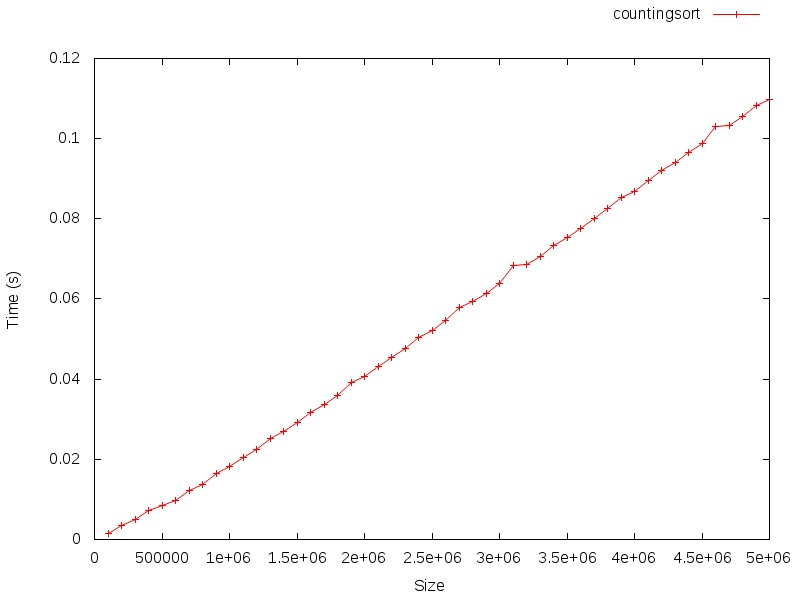
\includegraphics[scale=0.40]{images/countingsort.jpeg}
		\end{center}
	\end{alertblock}
\end{frame}

\begin{frame}{Comparación Ordenación por Conjuntos}
	\begin{alertblock}{}
		\begin{center}
		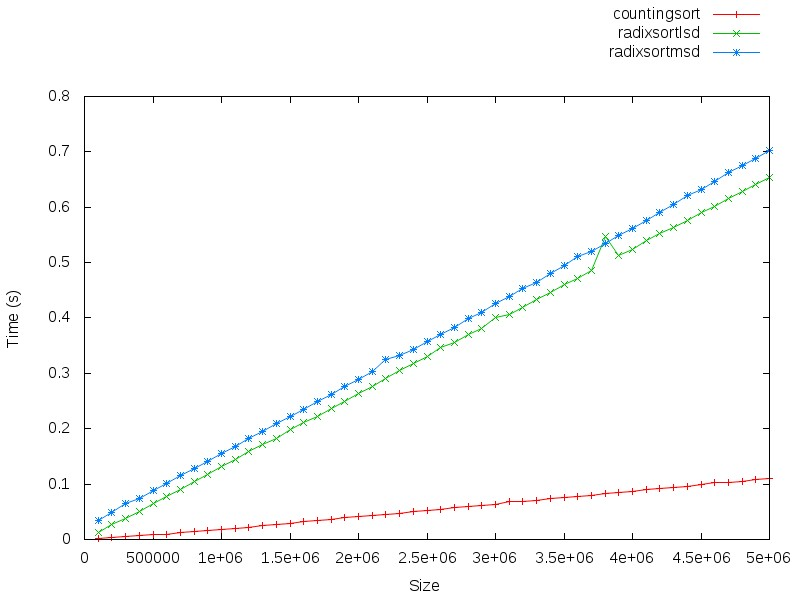
\includegraphics[scale=0.40]{images/coun-radi-radi.jpeg}
		\end{center}
	\end{alertblock}
\end{frame}

\begin{frame}{Comparación Countingsort-Quicksort}
	\begin{alertblock}{}
		\begin{center}
		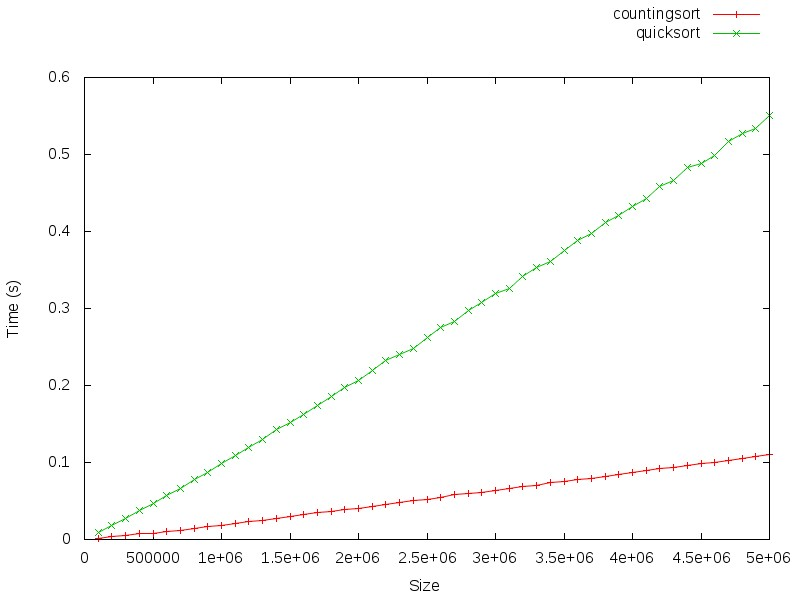
\includegraphics[scale=0.40]{images/coun-quic.jpeg}
		\end{center}
	\end{alertblock}
\end{frame}

\subsection{Varios}

\begin{frame}{Introducción}
En este apartado vamos a tratar algunos algoritmos que no encajan muy bien en las otras categorías, que no están implementados, o que simplemente son una chorrada que no merece mucho la pena prestarle atención.\\
\vspace{0.20in}
	\begin{exampleblock}{Nota}
	No hay gráficas de todos, solo de algunos.
	\end{exampleblock}
\end{frame}

\begin{frame}{Heapsort}
Vamos a empezar con el Heapsort, un algoritmo sumamente potente por el hecho de que trabaja muy bien con cualquier tipo de dato y es muy estable, a costa de algo menos de eficiencia (todo lo contrario que el Countingsort por ejemplo).\\
\vspace{0.20in}
La idea es meter todos los datos en un árbol binario parcialmente ordenado, que al volcarlo en el vector, estará ordenado. Implementar un árbol es tedioso, y explicarlo requiere de muchas horas, pero la STL puede ayudarnos en esta tarea proporcionándonos la priority\_queue (nos hará todo el trabajo sucio).\\
	\begin{block}{Eficiencia}
	La eficiencia de este algoritmo es siempre $\mathcal{O}(n\cdot\log_2(n))$, pues la inserción en el árbol es $\mathcal{O}(log_2(n))$ y hacemos $n$ inserciones.
	\end{block}
\end{frame}

\begin{frame}{Gráfica}
	\begin{alertblock}{}
		\begin{center}
		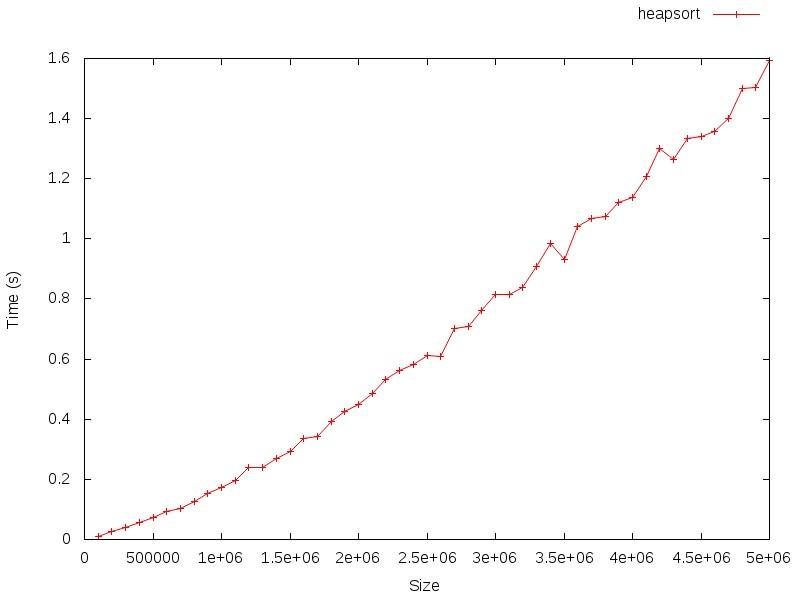
\includegraphics[scale=0.40]{images/heapsort.jpeg}
		\end{center}
	\end{alertblock}
\end{frame}

\begin{frame}{Comparación Mergesort-Heapsort}
	\begin{alertblock}{}
		\begin{center}
		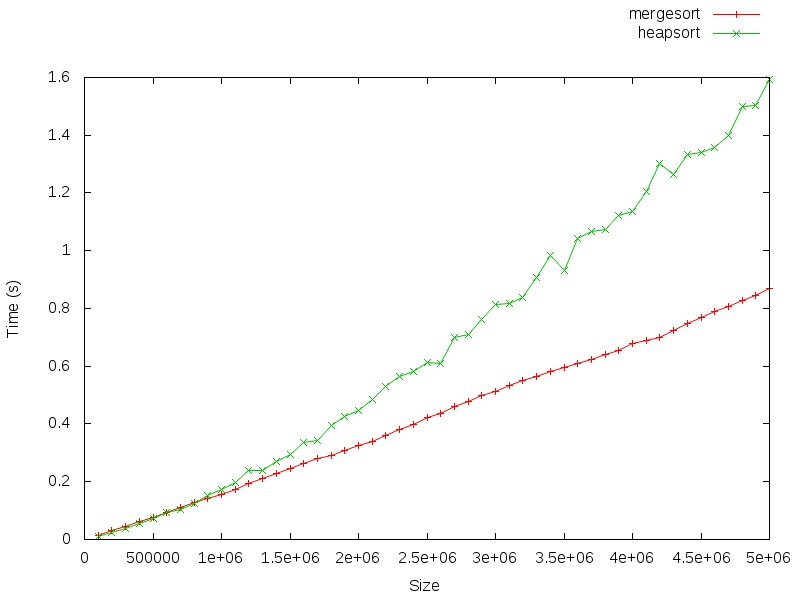
\includegraphics[scale=0.32]{images/merg-heap.jpeg}
		\end{center}
	\end{alertblock}
Como vemos, en rapidez no es mejor que el Mergesort.
\end{frame}

\begin{frame}{Timsort}
Se trata del algoritmo de ordenación que usan Python y OpenJDK.\\
\vspace{0.20in}
Es un algoritmo híbrido que hace uso del Mergesort y del Inserción para funcionar. Consiste básicamente en buscar sub-secuencias ordenadas (ya sea ascendente o descendentemente) y sabiendo eso, ordena el resto más eficientemente, usando Insertion cuando se pasa un umbral (normalmente $64$). Una vez ordenadas esas sub-secuencias, se aplica una fusión como la del Mergesort para ir obteniendo secuencias más grandes ordenadas.\\
\vspace{0.20in}
Con secuencias aleatorias suele ser peor, pero con secuencias de datos reales, el número de sub-secuencias ordenadas tiende a ser mayor, y es lo que aprovecha Timsort.
\end{frame}

\begin{frame}{Timsort}
	\begin{block}{Eficiencia}
	La eficiencia de este algoritmo es $\mathcal{O}(n\cdot\log_2(n))$, con mejores resultados en vectores parcialmente ordenados.
	\end{block}
\vspace{0.20in}
Una implementación de este algoritmo puede encontrarse en \href{https://github.com/gfx/cpp-TimSort}{github.com/gfx/cpp-TimSort}.\\
\vspace{0.20in}
Como se puede comprobar, no es algo precisamente trivial y requiere de muchas horas implementar algo así.
\end{frame}

\begin{frame}{Slowsort}
El nombre lo dice todo. Este algoritmo es más una curiosidad que otra cosa, una oda a como coger el camino más largo para resolver un problema.\\
\vspace{0.20in}
Básicamente consiste en ordenar las dos mitades del vector, quedarse con el mayor elemento de ambas mitades (el que está en la posición límite) y dejarlo al final del vector. Hecho esto, llamamos a Slowsort con todos los elementos menos el último. Simplemente absurdo.\\
	\begin{block}{Eficiencia}
	La eficiencia de este algoritmo es bastante compleja de calcular. De hecho no hay un orden exacto, aunque por aproximación se ha llegado a acotar por $\mathcal{O}(n^{\log_2(n)})$, aunque no es exacto.
	\end{block}
Ahora veremos en las gráficas por qué es tan malo.
\end{frame}

\begin{frame}{Gráfica}
	\begin{alertblock}{}
		\begin{center}
		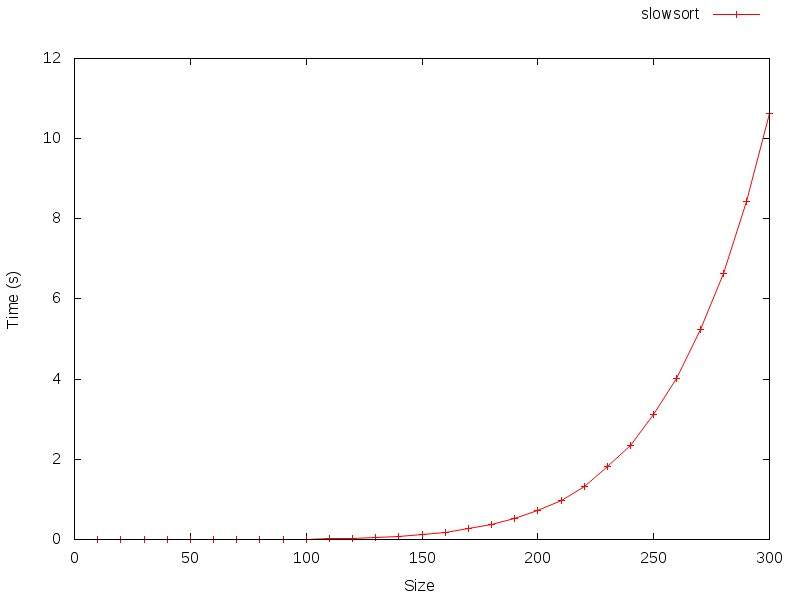
\includegraphics[scale=0.40]{images/slowsort.jpeg}
		\end{center}
	\end{alertblock}
\end{frame}

\begin{frame}{Comparativa Slowsort-Selección}
	\begin{alertblock}{}
		\begin{center}
		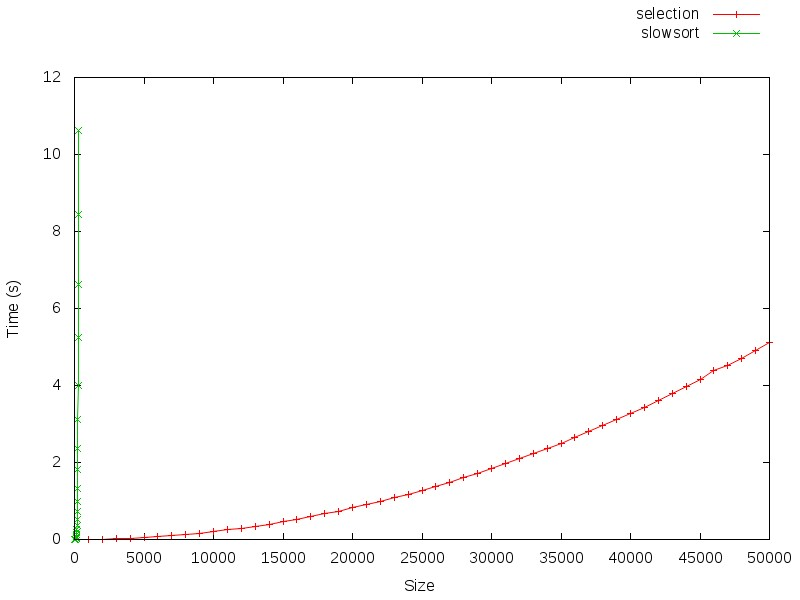
\includegraphics[scale=0.40]{images/sele-slow.jpeg}
		\end{center}
	\end{alertblock}
\end{frame}

\begin{frame}{Permutationsort}
Este algoritmo es muy simple de entender. Busca en todas las permutaciones posibles del vector (sin repetir permutaciones) hasta dar con la que esté ordenada.\\
\vspace{0.20in}
Puede optimizarse un poco si se evitan recorridos que seguro no llevan a la solución, cosa que es totalmente prescindible.\\
	\begin{block}{Eficiencia}
	Un vector de $n$ elementos tiene $n!$ permutaciones posibles. Dado que debemos comprobarlas todas y, por cada una, comprobar si está ordenada, la eficiencia se nos va a $\mathcal{O}(n\cdot n!)$, algo obviamente inviable para lo que ni hay gráfica (con 12 elementos tarda más de 10 segundos).
	\end{block}
\end{frame}

\begin{frame}{Bogosort}
Este algoritmo, también llamado Randomsort o Monkeysort, es igual que el anterior solo que puede repetir permutaciones.\\
\vspace{0.20in}
En efecto, genera una permutación aleatoria del vector y comprueba si está ordenada. En caso negativo, genera otra permutación (puede ser la misma o no).\\
	\begin{block}{Eficiencia}
	De media, la eficiencia es $\mathcal{O}(n\cdot n!)$, como el anterior, pero en el peor caso tiene eficiencia $\mathcal{O}(\infty)$, es decir, no asegura solución, por lo que ni podemos considerarlo un algoritmo.
	\end{block}
\end{frame}

\section{Final}

\begin{frame}{Final}
	\begin{center}
	{\Large Muchas gracias a todos por asistir}\\
	\vspace{0.30in}
	{\Huge Fin}
	\end{center}
\end{frame}
%%%%%%%%%%%%%%%%%%%%%%%
\end{document}
